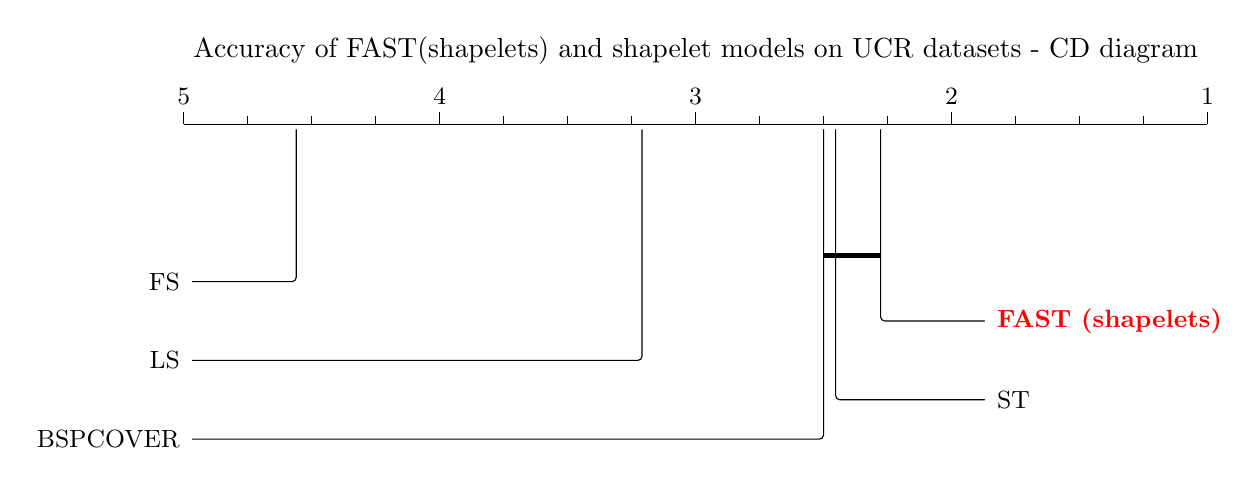
\begin{tikzpicture}[
  treatment line/.style={rounded corners=1.5pt, line cap=round, shorten >=1pt},
  treatment label/.style={font=\small},
  group line/.style={ultra thick},
]

\begin{axis}[
  clip={false},
  axis x line={center},
  axis y line={none},
  axis line style={-},
  xmin={1},
  ymax={0},
  scale only axis={true},
  width={13cm},
  ticklabel style={anchor=south, yshift=1.3*\pgfkeysvalueof{/pgfplots/major tick length}, font=\small},
  every tick/.style={draw=black},
  major tick style={yshift=.5*\pgfkeysvalueof{/pgfplots/major tick length}},
  minor tick style={yshift=.5*\pgfkeysvalueof{/pgfplots/minor tick length}},
  title style={yshift=\baselineskip},
  xmax={5},
  ymin={-3.5},
  height={3.5cm},
  xtick={1,2,3,4,5},
  minor x tick num={3},
  x dir={reverse},
  title={Accuracy of FAST(shapelets) and shapelet models on UCR datasets - CD diagram},
]

\draw[treatment line] ([yshift=-2pt] axis cs:2.277027027027027, 0) |- (axis cs:1.8603603603603605, -2.5)
  node[treatment label, anchor=west] {\textcolor{red}{\textbf{FAST (shapelets)}}};
\draw[treatment line] ([yshift=-2pt] axis cs:2.4527027027027026, 0) |- (axis cs:1.8603603603603605, -3.5)
  node[treatment label, anchor=west] {ST};
\draw[treatment line] ([yshift=-2pt] axis cs:2.5, 0) |- (axis cs:4.9774774774774775, -4.0)
  node[treatment label, anchor=east] {BSPCOVER};
\draw[treatment line] ([yshift=-2pt] axis cs:3.2094594594594597, 0) |- (axis cs:4.9774774774774775, -3.0)
  node[treatment label, anchor=east] {LS};
\draw[treatment line] ([yshift=-2pt] axis cs:4.5608108108108105, 0) |- (axis cs:4.9774774774774775, -2.0)
  node[treatment label, anchor=east] {FS};
\draw[group line] (axis cs:2.277027027027027, -1.6666666666666667) -- (axis cs:2.5, -1.6666666666666667);

\end{axis}
\end{tikzpicture}